\documentclass[a4paper,11pt]{article}
\usepackage{amsmath,amsthm,amsfonts,amssymb,amscd,amstext,vmargin,graphics,graphicx,tabularx,multicol} 
\usepackage[francais]{babel}
\usepackage[utf8]{inputenc}  
\usepackage[T1]{fontenc} 
\usepackage{pstricks-add,tikz,tkz-tab,variations}
\usepackage[autolanguage,np]{numprint} 

\setmarginsrb{1.5cm}{0.5cm}{1cm}{0.5cm}{0cm}{0cm}{0cm}{0cm} %Gauche, haut, droite, haut
\newcounter{numexo}
\newcommand{\exo}[1]{\stepcounter{numexo}\noindent{\bf Exercice~\thenumexo} : \marginpar{\hfill /#1}}
\reversemarginpar


\newcounter{enumtabi}
\newcounter{enumtaba}
\newcommand{\q}{\stepcounter{enumtabi} \theenumtabi.  }
\newcommand{\qa}{\stepcounter{enumtaba} (\alph{enumtaba}) }
\newcommand{\initq}{\setcounter{enumtabi}{0}}
\newcommand{\initqa}{\setcounter{enumtaba}{0}}

\newcommand{\be}{\begin{enumerate}}
\newcommand{\ee}{\end{enumerate}}
\newcommand{\bi}{\begin{itemize}}
\newcommand{\ei}{\end{itemize}}
\newcommand{\bp}{\begin{pspicture*}}
\newcommand{\ep}{\end{pspicture*}}
\newcommand{\bt}{\begin{tabular}}
\newcommand{\et}{\end{tabular}}
\renewcommand{\tabularxcolumn}[1]{>{\centering}m{#1}} %(colonne m{} centrée, au lieu de p par défault) 
\newcommand{\tnl}{\tabularnewline}

\newcommand{\bmul}[1]{\begin{multicols}{#1}}
\newcommand{\emul}{\end{multicols}}

\newcommand{\trait}{\noindent \rule{\linewidth}{0.2mm}}
\newcommand{\hs}[1]{\hspace{#1}}
\newcommand{\vs}[1]{\vspace{#1}}

\newcommand{\N}{\mathbb{N}}
\newcommand{\Z}{\mathbb{Z}}
\newcommand{\R}{\mathbb{R}}
\newcommand{\C}{\mathbb{C}}
\newcommand{\Dcal}{\mathcal{D}}
\newcommand{\Ccal}{\mathcal{C}}
\newcommand{\mc}{\mathcal}

\newcommand{\vect}[1]{\overrightarrow{#1}}
\newcommand{\ds}{\displaystyle}
\newcommand{\eq}{\quad \Leftrightarrow \quad}
\newcommand{\vecti}{\vec{\imath}}
\newcommand{\vectj}{\vec{\jmath}}
\newcommand{\Oij}{(O;\vec{\imath}, \vec{\jmath})}
\newcommand{\OIJ}{(O;I,J)}


\newcommand{\reponse}[1][1]{%
\multido{}{#1}{\makebox[\linewidth]{\rule[0pt]{0pt}{20pt}\dotfill}
}}

\newcommand{\titre}[5] 
% #1: titre #2: haut gauche #3: bas gauche #4: haut droite #5: bas droite
{
\noindent #2 \hfill #4 \\
#3 \hfill #5

\vspace{-1.6cm}

\begin{center}\rule{6cm}{0.5mm}\end{center}
\vspace{0.2cm}
\begin{center}{\large{\textbf{#1}}}\end{center}
\begin{center}\rule{6cm}{0.5mm}\end{center}
}



\begin{document}
\pagestyle{empty}
\titre{Contrôle 3 : Additions, soustractions et les cercles }{Nom :}{Prénom :}{Classe}{Date}


\exo{1,5} Compléter les pointillés en utilisant le bon vocabulaire (celui de la leçon) :\\

\bi
\item 73 est ..................................................... de 34 et de 39.\\
 
\item 33 et 12 sont ........................................................ de ........................................................... 33 - 12.\\
\ei

\exo{2} Poser et effectuer les opérations suivantes :               \\

\bmul{2}

294,75 + 4347,53

\vspace*{5cm}

\columnbreak

213,9 - 86,23	
\vspace*{5cm}

\emul

\exo{1,5} Calculer astucieusement avec la méthode vue en cours:\\

 R = 5,125 + 21 + 4,7 + 9 + 2,3 + 0,875 + 34\\
\reponse[5]\\



\exo{2} Entourer en bleu, pour chaque calcul, le meilleur ordre de grandeur :\\

\begin{tabular}{|c|c|c|c|c|}
\hline 
9,85 + 2,86 + 1,18 $\approx$& 10 & 15 & 14 & 20 \\ 
\hline 
489,45 + 968,90 + 204 + 75,90 $\approx$& 1 000 & 1 800 & 2 000 &  3 000 \\ 
\hline 
143,2 – 98,7 $\approx$ & 40 & 45 & 50 & 245 \\ 
\hline 
345,56 - 129,56 $\approx$& 200 & 480 & 210 &  230 \\ 
\hline 
\end{tabular} 

\vspace*{1cm}

\exo{2,5} Pour chaque problème, indiquer l'opération à effectuer pour le résoudre et écrire le résultat.


\begin{flushleft}
 
\includegraphics[scale=1]{tableau.eps}
 \end{flushleft} 



\exo{1}

Dans ce tableau, les sommes des nombres doivent toujours être égales sur chaque ligne, chaque colonne et chaque diagonale.\\

\begin{center}
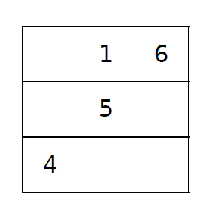
\includegraphics[scale=1]{carre.eps} 
\end{center}




\end{document}
